\documentclass[12pt,table,t]{beamer}

% Packages
\usepackage[norsk]{babel}
\usepackage[utf8]{inputenc}

% Theme
\mode<presentation>
{
  \usetheme{Honefoss}
  \setbeamertemplate{blocks}[rounded]
}

\newcommand{\comment}[1]{{\slshape\color{kvred}#1}}
\setbeamertemplate{caption}{\raggedright\insertcaption\par}

\title{Lasermålinger mot satellitter}
\subtitle{}
\author{Ingrid Fausk}
\date{Geodesi- og hydrografidagene, 27. november 2019}

\begin{document}
\frame[plain]{\titlepage}

\begin{frame}{Kartverkets ambisjoner innen SLR}
  \framesubtitle{Satellite Laser Ranging}
  \vspace{0.7cm}
  \begin{columns}
    \column{0.45\textwidth}
      \includegraphics[width=0.95\textwidth]{figure/jordklode.eps}
    \column{0.45\textwidth}
      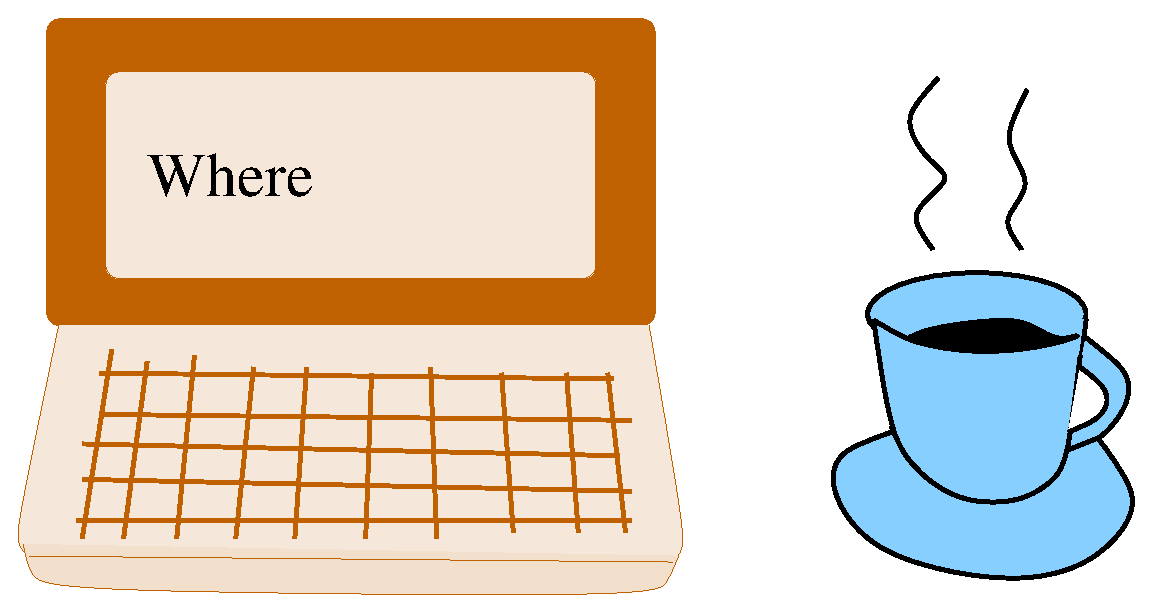
\includegraphics[width=0.95\textwidth]{figure/where.eps}
  \end{columns}
\end{frame}


\begin{frame}{Retroreflektorer}
  \begin{tabular}{cl}
    &  \\
    \raisebox{-.5\height}{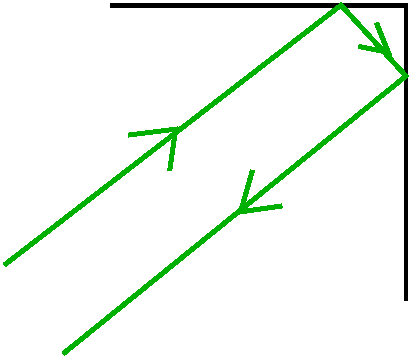
\includegraphics[width=0.2\textwidth]{figure/laser.eps}} & 
    \begin{minipage}[t]{0.6\columnwidth}Lyset reflekteres i samme retning som det kom fra \end{minipage}\\
    &  \\     
    \raisebox{-.5\height}{\includegraphics[width=0.2\textwidth]{figure/plotkin_-_beacon_explorer_a2.jpg}} & 
    \begin{minipage}[t]{0.6\columnwidth}Første satellitt med retroreflektorer, Beacon Explorer B, 1964. Henry Plotkin undersøker reflektorene.\end{minipage}\\
  \end{tabular}
\end{frame}


\begin{frame}{LAser GEOdynamics Satellite}
  \begin{columns}
    \column{0.6\textwidth}
      \begin{itemize}
        \item LAGEOS-1, 1976 (USA)
        \item LAGEOS-2, 1992 (Italia)
        \item Vekt: 400 kg
        \item Omløpstid: 220 min
        \item Høyde: 5800 km
        \item Diameter: 60 cm
        \item Levetid: 8.4 mill år. Inneholder en tidskapsel. 
      \end{itemize}
    \column{0.3\textwidth}
      \begin{figure}
        \includegraphics[width=0.7\textwidth]{figure/lageos_1.jpg} \caption{Photo: NASA}
      \end{figure}
  \end{columns}
\end{frame}


\begin{frame}{Stasjonsnettverk}
  \begin{figure}
    \includegraphics[width=0.9\textwidth]{figure/slrmap.png}\caption{Grafikk: NASA}
  \end{figure}
\end{frame}


\begin{frame}{Ny Ålesund}
  \framesubtitle{SLR ferdigstilles i 2024, bygges av NASA}
  \begin{figure}
    \includegraphics[width=0.9\textwidth]{figure/PAB_jordobservatoriet.jpg}\caption{Foto: Per Anders Bjørklund}
  \end{figure}
\end{frame}


\begin{frame}{Banen til LAGEOS-1}
  \begin{figure}
    \includegraphics[width=0.9\textwidth]{figure/orbit_l1_4h.png}\caption{Bare 5 stasjoner målte mot Lageos1 i første omløp 1. oktober 2019. Banen er beregnet med {\it Where}.}
  \end{figure}
\end{frame}


\begin{frame}{Banen til LAGEOS-1}
  \begin{figure}
    \includegraphics[width=0.9\textwidth]{figure/orbit_l1_week.png}\caption{26 stasjoner målte mot Lageos1 i perioden 1. - 7. oktober 2019. Banen er beregnet med {\it Where}.}
  \end{figure}
\end{frame}


\begin{frame}{ITRF}
\framesubtitle{International Terrestrial Reference Frame}
  \begin{description}
    \item[Hvorfor?] For å kunne måle platetektonikk, havnivå masseforflytninger etc. i referanse til noe
    \item[Hvordan?] Laget ved hjelp av fire geodetiske teknikker GPS, VLBI, SLR og DORIS
    \item[Når?] Må oppdateres jevnlig, fordi vi har nye modeller, nytt måleutstyr, og fordi jorda forandrer seg
    \item[Sist gang:] ITRF2014
    \item[Neste gang:] ITRF2020
  \end{description}
\end{frame}


\begin{frame}{Referanserammen}
  \begin{columns}
    \column{0.22\textwidth}
      \vspace{0.9cm}
      \begin{figure}
        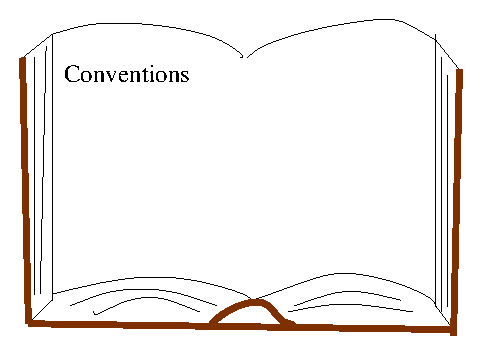
\includegraphics[width=0.95\textwidth]{figure/book.eps}\caption{Regelboken}
      \end{figure}
    \column{0.08\textwidth}\\ \ \\ \ \\ \ \\ \ \\ 
      +  
    \column{0.22\textwidth}
      \begin{figure}
        \includegraphics[width=0.95\textwidth]{figure/jordklode.eps}\caption{Observasjoner}
      \end{figure}
    \column{0.08\textwidth}\\ \ \\ \ \\ \ \\ \ \\
      =
    \column{0.26\textwidth}
      \\ \ \\ 
      \begin{figure}
        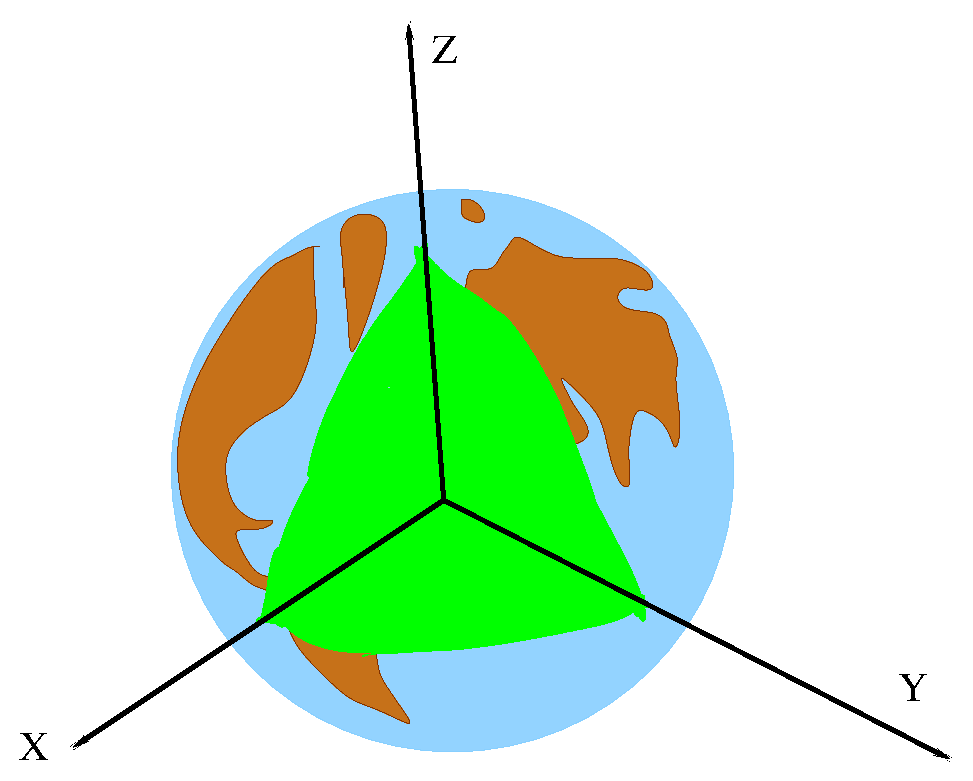
\includegraphics[width=0.97\textwidth]{figure/referanseramme.eps}\caption{Referanserammen}
      \end{figure}
  \end{columns}
\end{frame}


\begin{frame}{Jordrotasjonsparametre}
  \begin{center}
    \begin{figure}
      \includegraphics[width=0.15\textwidth]{figure/eop_parameters.png}
    \end{figure}

  \begin{figure}
    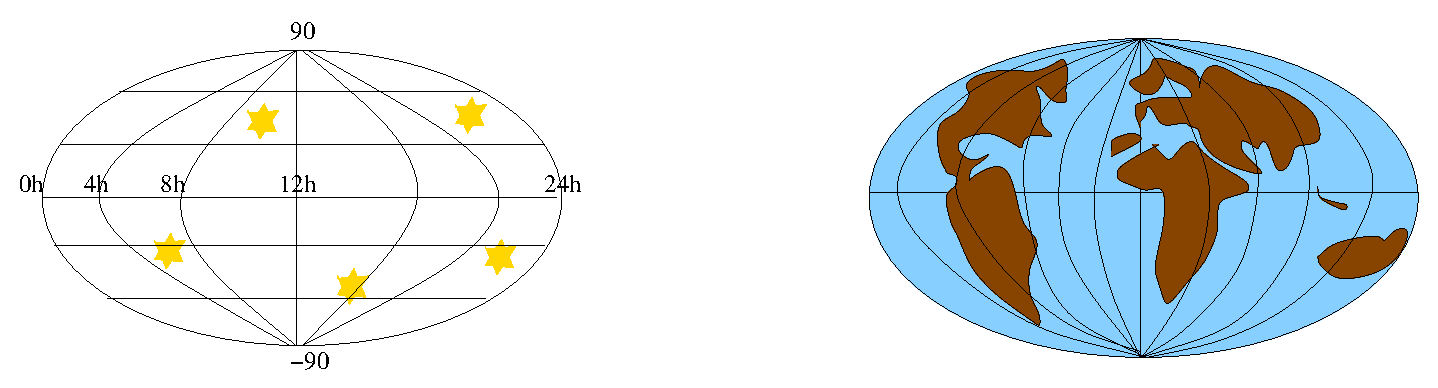
\includegraphics[width=0.8\textwidth]{figure/eop.eps}\caption{Hvordan jordfast system er rotert i forhold til himmelfast system.}
  \end{figure}
  \end{center}
\end{frame}


\begin{frame}{Verdikjeden for SLR}
\framesubtitle{(og hvor Kartverket vil være med og bidra i fremtiden)}
  \begin{tabular}{clc}
    &  \\
    \fbox{40+ stasjoner med SLR} & \includegraphics[width=0.08\textwidth]{figure/pil_horisontal.eps}  & \fbox{
          \includegraphics[width=0.1\textwidth]{figure/kartverket.png}}\\

    
\includegraphics[width=0.015\textwidth]{figure/pil.eps} && \\

    \fbox{2 datasentre i USA/Tyskland} && \\

    
\includegraphics[width=0.015\textwidth]{figure/pil.eps} && \\
    \fbox{7 analysesentre} & \includegraphics[width=0.08\textwidth]{figure/pil_horisontal.eps} &  \fbox{
          \includegraphics[width=0.1\textwidth]{figure/kartverket.png}}\\

    
\includegraphics[width=0.015\textwidth]{figure/pil.eps} && \\
    \fbox{2 kombinasjonssentre i USA/Italia} & &\\
  \end{tabular}
\end{frame}


\begin{frame}{Verdikjeden for referanserammen}
\framesubtitle{International Earth Rotation and Reference Systems Service (IERS) koordinerer arbeidet}
  \begin{tabular}{clc}
    &  \\
    \fbox{VLBI + SLR + GNSS + DORIS + Local Ties} \\

    
\includegraphics[width=0.015\textwidth]{figure/pil.eps} \\

    \fbox{Kombinasjon i Tyskland/Frankrike/USA} \\

    
\includegraphics[width=0.015\textwidth]{figure/pil.eps} \\

    \fbox{ITRF: International Terrestrial Reference Frame}

  \end{tabular}
\end{frame}


\begin{frame}{Korreksjoner}
  \begin{itemize}
    \item Betyr ikke at målingen er «feil»
    \item I SLR måler vi gangtiden til signalet, ikke faktisk avstand
    \item Forsinkelse av signalet gjennom atmosfæren utgjør 3-4 meter
    \item Signalet reflekteres ikke i sentrum av satellitten
    \item Stasjonsforflytning: Tidekrefter etc.
  \end{itemize}
\end{frame}


\begin{frame}{Baneberegning}
  \begin{itemize}
    \item Analysesentrene beregner sine egne baner
    \item Iterativ prosess, numerisk integrasjon
    \item Må ta hensyn til alle krefter som virker på satellitten
    \item Minste kvadraters metode tilpasning til målingene
    \item Bruker banen som en «fast referanse i rommet», regner ut korreksjoner for stasjonsposisjonene etterpå
  \end{itemize}
\end{frame}


\begin{frame}{Where}
  \framesubtitle{Vår programvare for geodetisk analyse}
  \begin{itemize}
    \item Utvikles ved Kartverket
    \item Skrives i Python
    \item Testleveranser til International VLBI Service pågår
    \item Plan om testleveranser også til International Laser Ranging Service i løpet av 2020
    \item Har som målsetning å bli analysesenter for VLBI og SLR
  \end{itemize}
  \begin{center}
    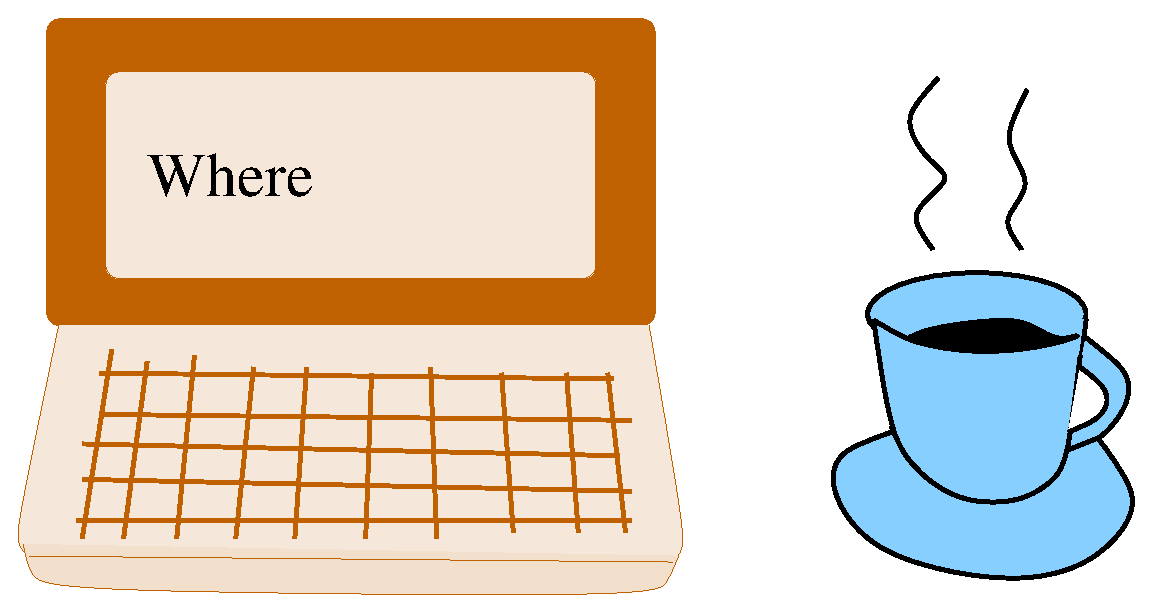
\includegraphics[width=0.3\textwidth]{figure/where.eps}
  \end{center}
\end{frame}

\end{document}
